\subsection{Reduced model verification}

The model derived in \cref{sec:kalman} is to be used as an observer for the system. Control signals will be calculated using the esimated states from this model. To verify the model, it is initially tested as an observer to the larger model from \cref{sec:mod_lin}.\\

A Luenberg observer gain has been designed to ensure accuracy in the estimated output of the reduced model. Any error between the actual output and estimated output will be multiplied by L and added to the $\dot{\hat{x}}$. If $A-LC$ is stable, this topology will ensure $y = \hat{y}$ and if the states are observable (which the Kalman Decomposition ensures they are) $x=\hat{x}$. This is only true in the absence of disturbances. If any such are present, the proportional observer gain will not be sufficient to estimate the states, and integral action should be included.

The observer poles $\text{eig}(A-LC)$ are chosen to be have the same angle as the closed loop poles $\text{eig}(A-BK)$ but with a 5 times larger magnitude. This ensures the observer is always faster then the system dynamics, and nothing happens with $x$ that is not clear by looking the observer states $\hat{x}$.\\

For the test all states $x$ are initialised with the value 1. This is an arbitrary value, and merely chosen to verify that all states are driven to zero, and the observed state vector $\hat{x}$ converges to $x$. We briefly recall that in this coordinate system $x=0$ physically means $x-x_o = 0 \rightarrow x=x_o$. The control signal u is defined as $u=K\hat{x}$.\\

In \cref{fig:sim_modelSS_obs} the Matlab Simulink simulation model is seen. In \cref{fig:sim_stateInput30h} a plot containing the states and inputs is seen. The simulation has run for 30 hours. In \cref{fig:sim_stateInput1h} the same plot is seen but zoomed in at 1 hour such that the behavior of the states is more easily observed. In \cref{fig:sim_stateObsState1h} The states are compared to the observed states at the same time zoom level as the previous plot. In \cref{fig:sim_stateObsState002h} further zoom is made on the time axis to observe the fast transients in the first seconds of the simulation where the observer converges from the big starting error.

\begin{figure}[h!]
	\centering
	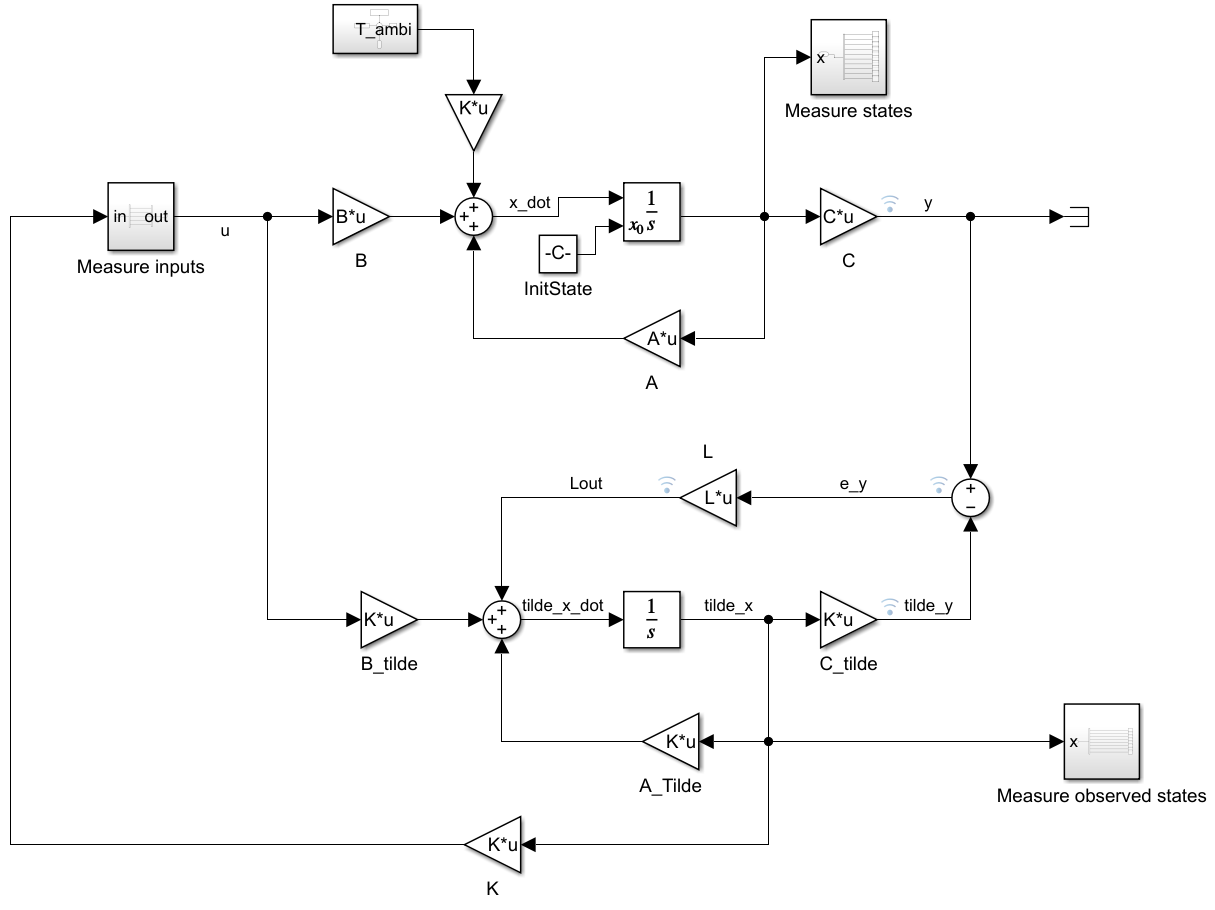
\includegraphics[width=1\textwidth]{Graphics/fig_modelSS_obs.png}
	\caption{The Matlab Simulink simulation model of the linearised system with feedback from Kalman Decomposition observer}
	\label{fig:sim_modelSS_obs}
\end{figure}

\begin{figure}[h!]
	\centering
	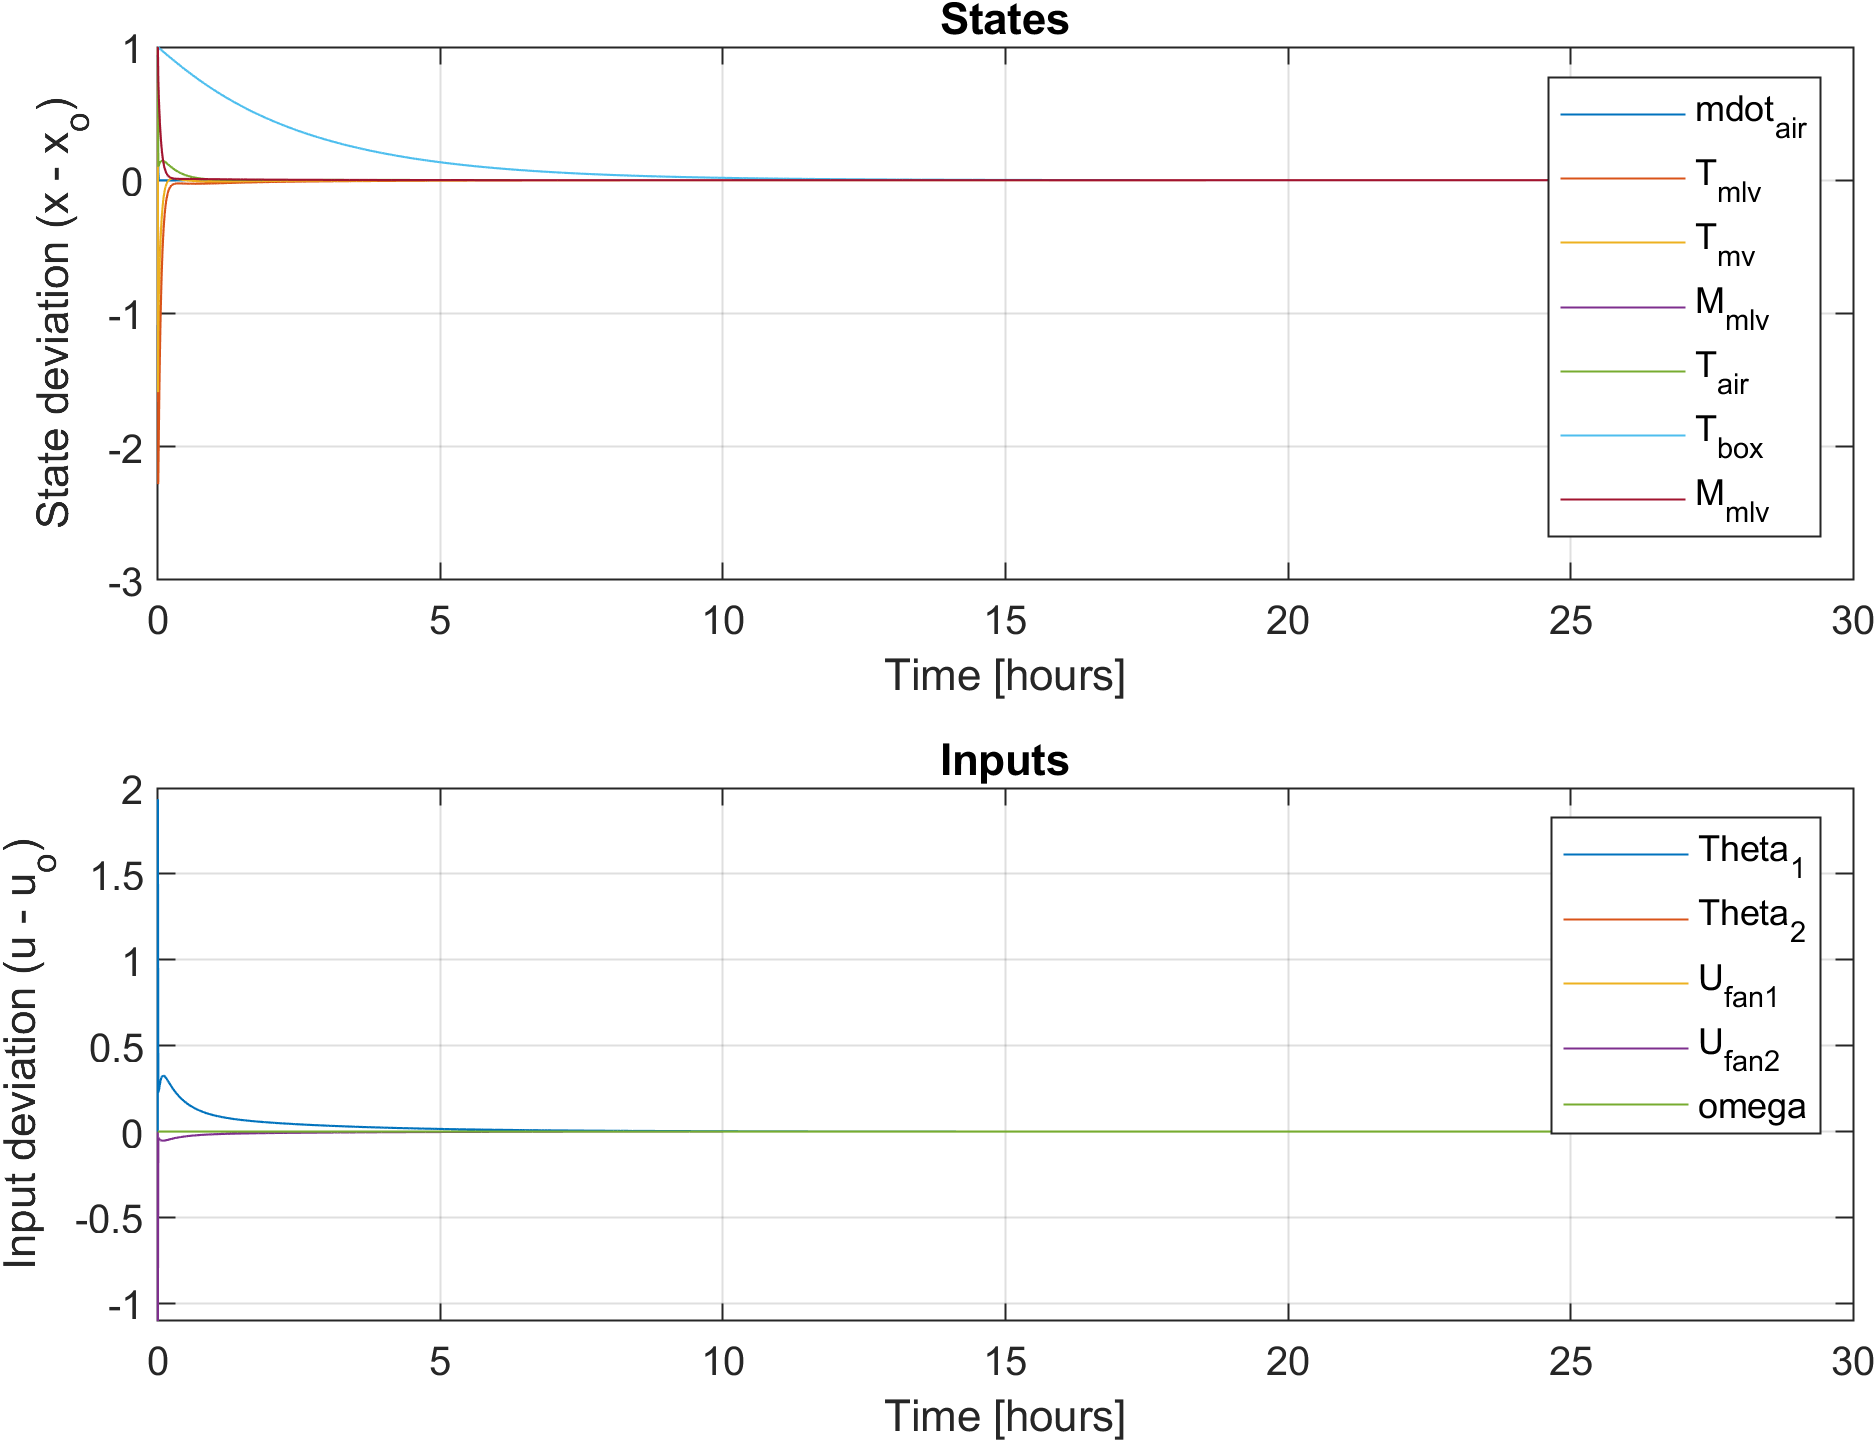
\includegraphics[width=0.7\textwidth]{Graphics/fig_stateInput30h.png}
	\caption{States and the inputs for 30 hours}
	\label{fig:sim_stateInput30h}
\end{figure}

\begin{figure}[h!]
	\centering
	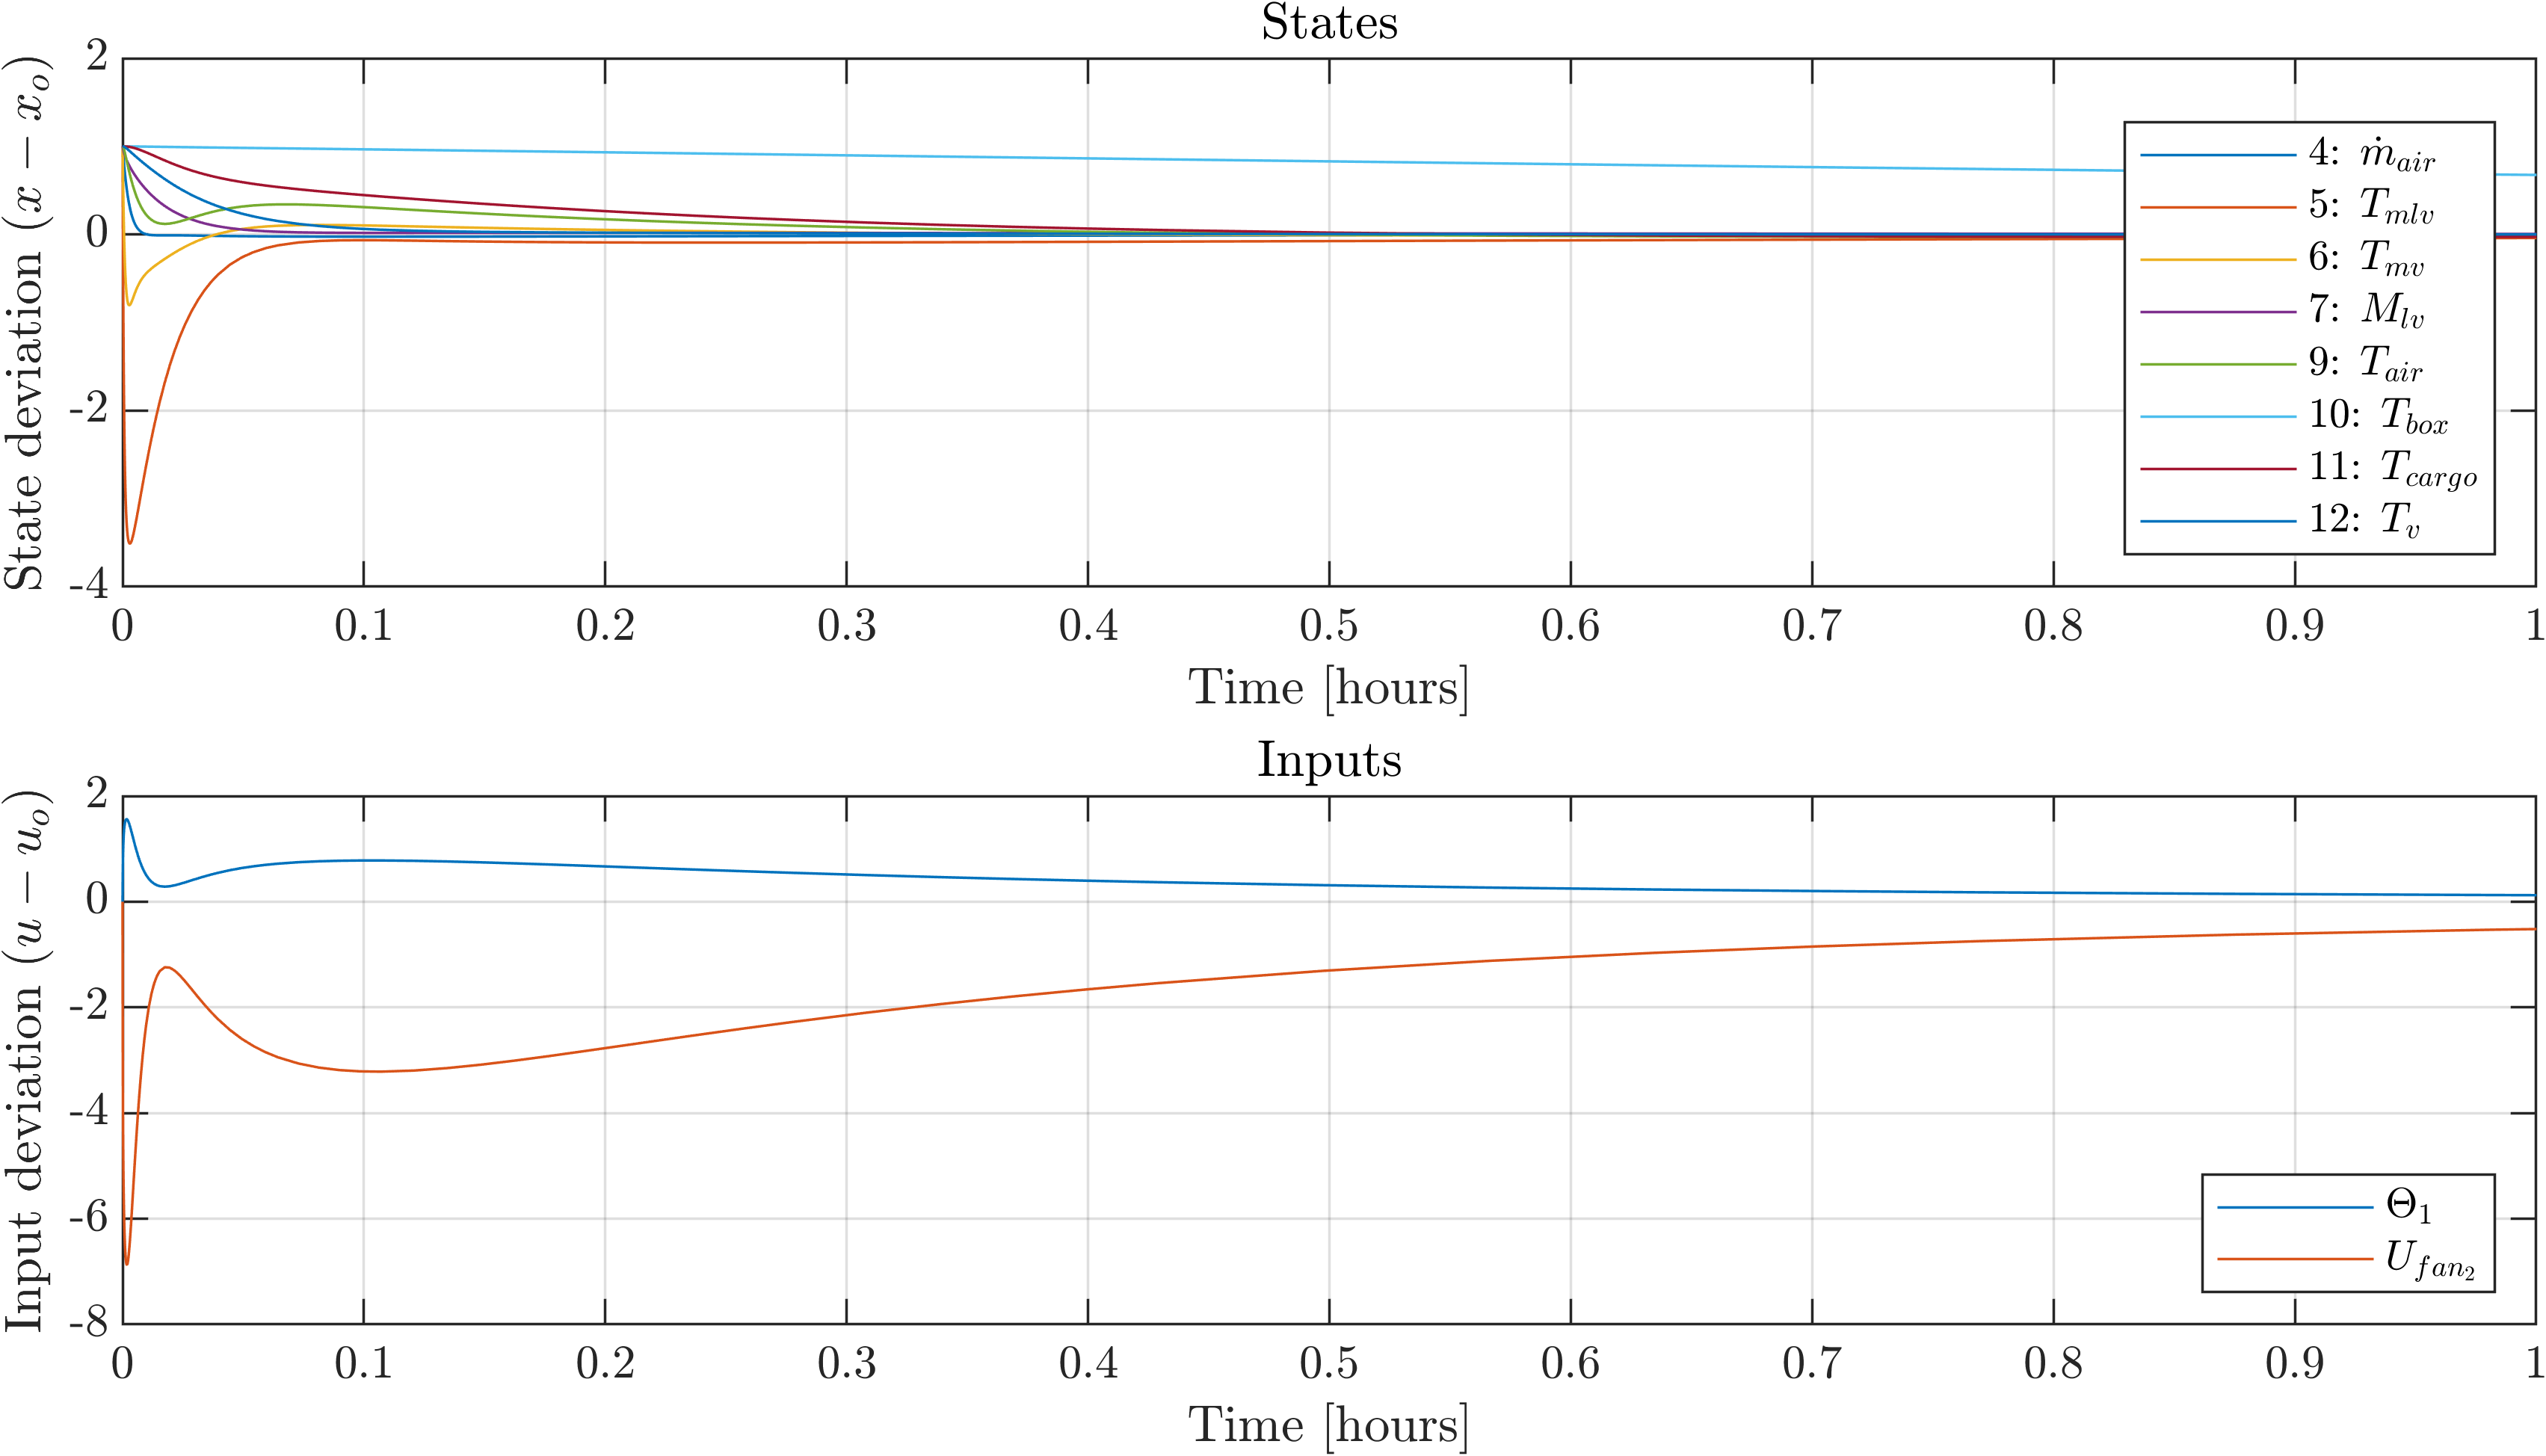
\includegraphics[width=0.7\textwidth]{Graphics/fig_stateInput1h.png}
	\caption{States and the inputs for 1 hour}
	\label{fig:sim_stateInput1h}
\end{figure}

\begin{figure}[h!]
	\centering
	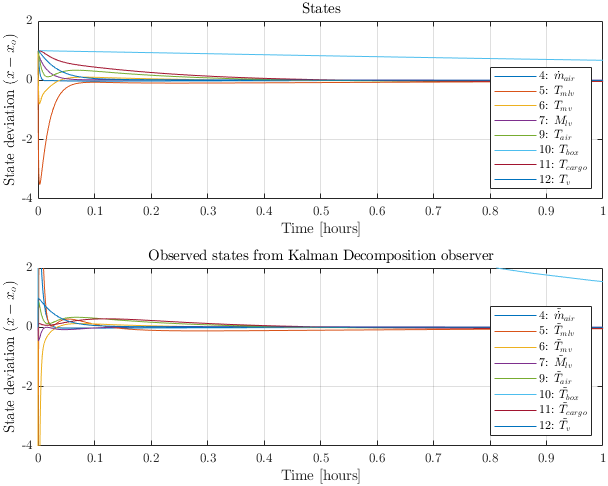
\includegraphics[width=0.7\textwidth]{Graphics/fig_stateObsState1h.png}
	\caption{States and Kalman Decomposition observers observed states for 1 hour}
	\label{fig:sim_stateObsState1h}
\end{figure}

\begin{figure}[h!]
	\centering
	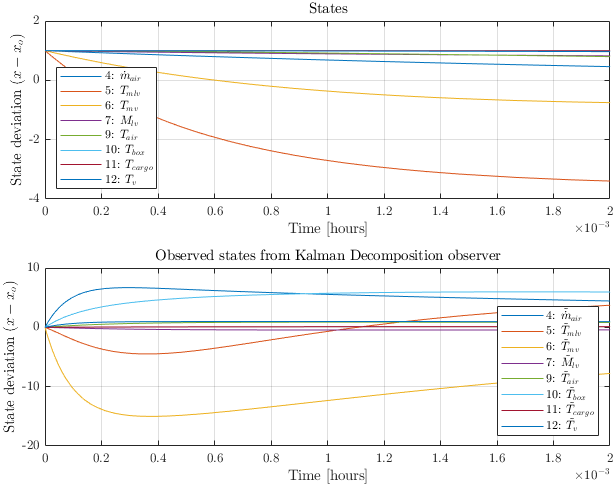
\includegraphics[width=0.7\textwidth]{Graphics/fig_stateObsState002h.png}
	\caption{States and Kalman Decomposition observers observed states for 0.002 hours}
	\label{fig:sim_stateObsState002h}
\end{figure}
